\documentclass[main.tex]{subfiles}
\begin{document}

\chapter{Results}\label{ch:results}

\section{Data Sets}
\subsection{Overview and Comparison}
The data presented here were collected during a one-hour measurement with both the analog and the digital setup running in parallel. A total of 4.3 million pulses from the NE213 detector were recorded by the analog setup. The digitizer saw 2.2 million pulses from the NE213 detector. This large difference in counts was because the digital setup was configured to transfer each event individually, resulting in a very low livetime.

In the analog setup, thresholds of -25.0 mV and -94.6 mV were applied to the YAP detector and the NE213 detector, respectively. In the digital setup, thresholds of -9.8 mV and -48.8 mV were applied to the YAP and the NE213 detector, respectively. Having such a low threshold on the YAP was found to decrease the signal-to-noise ratio in the ToF spectrum, so a higher threshold of -24.4\si{\milli\volt} was applied in software. Table \ref{tab:settings} presents an overview of the datasets.
\begin{table}[bh]
\begin{tabular}{|l|l|l|l|l|}
\hline
Setup   & YAP threshold (mV) & NE213 threshold (mV) & NE213 events ($\text{10}^\text{6}$) & Livetime \\ \hline
Analog  & -25.0              & -94.6                & 4.3      & 44\%             \\ \hline
Digital & -9.8/-24.4*			& -48.8                & 2.2      & **             \\ \hline
\end{tabular}
\caption[Overview of the analog and digital data sets.]{Overview of the analog and digital data sets. *A threshold of \SI{24.4}{mV} was enforced offline (see text for details). **The digital setup did not have a method for determining livetime.}
\label{tab:settings}
\end{table}



\subsection{Livetime and threshold alignment}
\subsubsection{Deposited energy}
The analog and the digital setups were run with different amplitude thresholds. To properly compare them, a common threshold was necessary. Further, the analog and digital setups have significantly different cable lengths to the detectors. Thus, the signals were attenuated differently before being processed by the different systems. As a result, the required digital-setup threshold was significantly higher than the analog threshold.

\begin{figure}[h!]
    \centering
        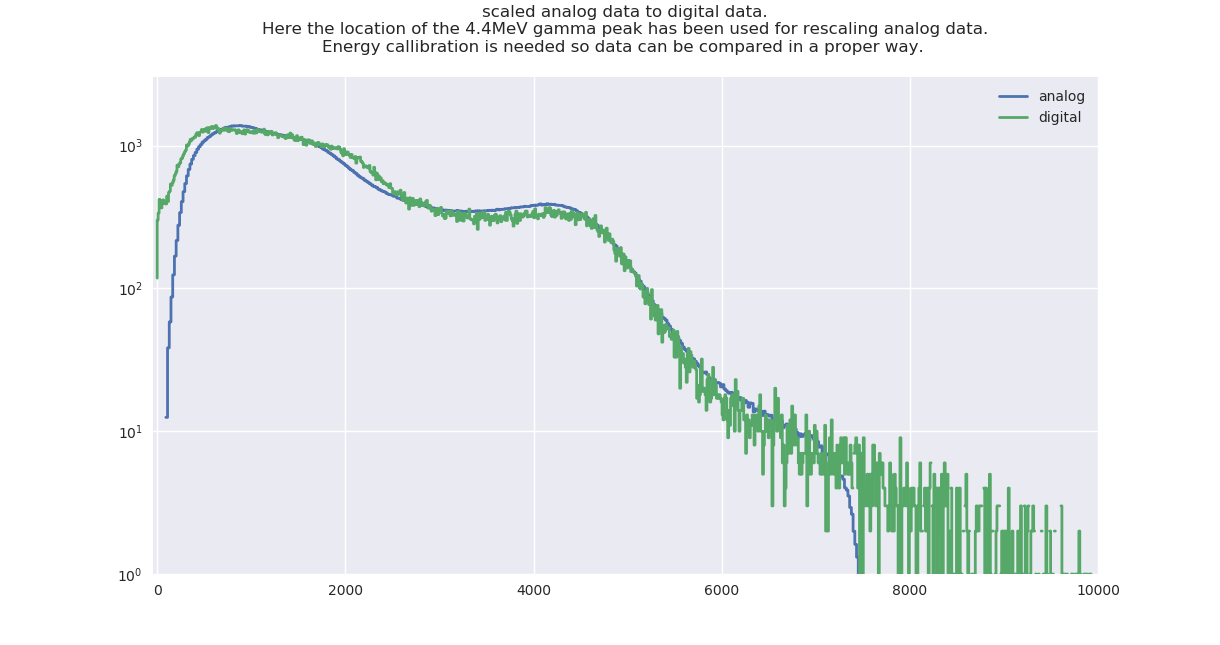
\includegraphics[width=0.7\textwidth]{CompareResults/qdc_comp.pdf}
        \caption[Comparison of analog and digital spectra from the NE213 detector]{Comparison of analog and digital spectra from the NE213 detector. Top: The red histogram is the livetime-corrected analog energy spectrum. The blue histogram is the raw digital energy spectrum and the green histogram is the digital energy spectrum after threshold matching and normalization. Bottom: ratio of counts between livetime-corrected analog spectrum and normalized digital spectrum.}
    \label{fig:qdc_comp}
\end{figure}
Figure~\ref{fig:qdc_comp} top panel shows the energy spectra from both setups. The data from the analog setup have been livetime corrected (44\%). The blue histogram shows the raw digital spectrum, and the green histogram shows the digital spectrum after applying a higher amplitude threshold of \SI{-151}{mV} in software and normalizing the spectrum to match the height of the livetime-corrected analog setup. The resulting spectra are far more similar but, although the Compton edges associated with the \SI{4.44}{\MeV}$_\text{ee}$ gamma-ray do not look the same. This may be because some of these gamma-rays deposited energies which exceeded the dynamic range of the digitizer. 
The livetime of the digital setup can be estimated by multiplying the analog setups livetime to the ratio of counts in the digital and analog setups. This provides a crude estimate of 22\% of the digital setups livetime.

Figure~\ref{fig:qdc_comp} bottom panel shows the ratio between the digital and analog spectra after threshold alignment and normalization. Ideally this ratio should be unity. This is not the case. Near the Compton edge corresponding to the \SI{4.44}{\MeV}$_\text{ee}$ gamma-ray there is a bump and a valley, indicated with arrows in the figure. Again this may be due to the highest amplitude digitized pulses corresponding to the highest energy Compton events being clipped, causing them to register lower values of deposited energy.


\subsubsection{Time-of-flight spectra}
The ToF spectrum is heavily influenced by the choice of amplitude threshold. Figure~\ref{fig:tof_comp} top panel shows ToF spectra for the two setups with the initial -49 mV NE213 detector threshold on the digital setup and -94.6 mV on the analog setup. Interestingly it seems that the analog setup misses the slower neutrons due to the high amplitude threshold. By applying the offline NE213 detector threshold of \SI{-151}{mV} and the YAP detector threshold of \SI{-44}{mV} to the digital setup and normalizing the data as before, the ToF spectra shown in the bottom panel of Fig.~\ref{fig:tof_comp} are obtained. The neutron peaks now have roughly the same shape, which means that the amplitude cut has removed the slower neutrons.

\begin{figure}[h]
    \centering
        \includegraphics[width=0.7\textwidth]{CompareResults/tof_comp.pdf}
        \caption[Analog and digital time-of-flight spectra.]{Analog and digital time-of-flight spectra. Top: Unadjusted. Bottom livetime has been taken into account and a higher threshold has been enforced on the NE213 and YAP signals for the digital setup.}
    \label{fig:tof_comp}
\end{figure}

\section{Analog Setup}

\subsection{Neutron Tagging}
Figure~\ref{fig:tof_a} shows the ToF spectrum recorded by the analog setup. The neutron and gamma-ray peaks are marked with arrows. In addition to these two peaks, there is an approximately flat background. This background represents uncorrelated particles triggering the TDC start and stop, which is also why negative ToF values appear.
The gamma-flash has been shifted to be centered at \SI{3.8}{ns}, the time it takes light to travel from source to detector. The width of the gamma-flash is primarily due to the time resolution of the detectors. This depends on where in the detector volume the gamma-ray interacts. Secondary effects include signal attenuation in the cables, which might affect PS and thus rise time. This may in turn make the CFD less effective and may cause loss in the time resolution. Furthermore, the final  digitization by the TDCs may cause some loss of resolution. Differences in flight path between gamma-rays hitting the center of the NE213 and those that hit near the edge will be less than \SI{1}{cm}, so this will not give rise to a substantial time spread. 
\begin{figure}[ht]
    \centering
        \includegraphics[width=0.9\textwidth]{AnalogResults/tof.pdf}
        \caption[Time of flight spectrum, analog setup.]{The time of flight spectrum. The x-axis denotes the time of flight from source to NE213 detector. The neutron and gamma peaks have been indicated with arrows. The coincidences highlighted in red have been converted to neutron kinetic energies and are shown in the upper right insert.}
    \label{fig:tof_a}
\end{figure}
The neutron bump has faster neutrons at lower ToF values and slower neutrons at higher ToF values. Since the distance from the source to the detector is known, it is possible to convert the neutron ToF into neutron kinetic energy. A range of $1.5\--7$~\si{\MeV} was used. This corresponds to a time interval of $31\--$\SI{68}{\ns}. The coincidences falling in this time interval have been highlighted in red in Fig.~\ref{fig:tof_a} and the corresponding energies are shown in the insert. The spectrum obtained by Scherzinger~\cite{ScherzingerPhd} (recall Fig.~\ref{fig:scherzinger}) has been superimposed. This spectrum has ben normalized to get the the best qualitative agreement possible. The Scherzinger spectrum was produced with the same source but a different and smaller NE213 detector. This detector had only $\sim10\%$ of the scintilation volumne of the one applied here. 
Comparing with Scherzingers spectrum it appears that the slower neutrons are missing. This is likely because a too large amplitude threshold has been applied. 
It also appears that the neutron energy spectrum acquired by the analog setup is shifted to the right by rougly half an MeV. Below \SI{2.5}{MeV} the count rate in Fig.~\ref{fig:tof_a} increases. This is simply an effect of the last $\sim$\SI{20}{\ns} primarily consisting of background, and that the lowest energies covers a wider range of flight times since $E\propto \dfrac{1}{ToF^2}$.



\subsection{Pulse-Shape Discrimination}
Neutrons and gamma-rays were discriminated using the PS parameter given in Eq.~\ref{eq:ps}. The parameters $a$=120 QDC channels and $b$=0 QDC channels were found to linearize PS as a function of energy, when gate lengths of \SI{500}{\ns} and \SI{60}{ns} were used for the LG and SG integrations respectively.
PS is shown as a function of deposited energy in Fig.~\ref{fig:psd_a}. Pulses in the upper band labeled neutrons have a large amount of charge in the tail of the scintilation pulse. Pulses in the lower band labeled gamma-rays have a smaller amount charge in the tail of the scintillation pulse. 
This is confirmed by the presence of the Compton edges corresponding to \SI{2.23}{MeV} and \SI{4.44}{MeV} gamma-rays in the lower band. The amplitude threshold of \SI{-94.6}{mV} gives rise to the sloping energy threshold highlighted with a red line in the figure. This is because pulses with higher PS  have more charge in tail, so given two pulses of equal amplitude the one will larger PS will carry more charge.
\begin{figure}[ht]
    \centering
        \includegraphics[width=\textwidth]{AnalogResults/psd_a.pdf}
        \caption[Analog pulse-shape spectrum as a function of deposited energy.]{Analog pulse-shape spectrum as a function of deposited energy. The dashed white line indicates the PSD cut. Structures due to the \SI{2.23}{MeV} and \SI{4.44}{MeV} gamma-rays are indicated. The red line indicates the amplitude threshold.}
        \label{fig:psd_a}
\end{figure}

The optimal PS-cut value of 0.259 was found by plotting a PS histogram and fitting Gaussian functions to the neutron and gamma-ray distributions, see~\ref{fig:fom_a}. The quality of separation between the two distributions may be expressed as a Figure of Merit, FoM, defined in terms of the centers, C, of the Gaussian functions and their full width at half maximum, W. Figure~\ref{fig:fom_a} shows histograms of the PS parameter along with the Gaussian fits used to calculate the FoM. The corresponding parameters are listed in Table \ref{tab:fom_a}. The resulting FoM was 0.58, but it was found to be highly energy threshold dependent\footnote{For more information on the energy dependence of the FoM, see Appendix \ref{ch:appA}.}. 

The neutron and gamma-ray distributions overlap at low deposited energies. Consequently, the PSD cut can result in misclassification. Orthogonal ToF information on particle species can be used to quantify the extent of this misclassification.
Figure~\ref{fig:tof_ps_a} shows PS plotted as a function of ToF, with neutron and gamma-ray distributions highlighted. 
These distributions are not cleanly separated by the applied PSD cut. A significant amount of both neutrons and gamma rays are mislabeled. Often the start and stop signal will be due to uncorrelated particles, rather than the previously discussed $n\gamma$ and $\gamma\gamma$ pairs. These events are expected to form a flat background in the ToF spectrum, due to low rates. This may be seen in Fig. \ref{fig:tof_a} at times longer than\SI{50}{ns}. Since the events still represent either neutrons or gamma-rays (ignoring the occasional muon) one would expect them to be clearly separated into two bands in Fig.~\ref{fig:tof_ps_a}. Neutrons at slightly higher PS value and gamma rays at lower PS value. This is not the case.

\begin{equation}
FoM = \frac{C_n - C_\gamma}{W_n + W_\gamma},
\end{equation}
\begin{figure}[h!]
	    \centering
    	    \includegraphics[width=0.8\textwidth]{CompareResults/FOM_analog.pdf}
    \caption[Pulse shape figure of merit for the analog setup.]{Pulse shape figure of merit for the analog setup. The inset shows the pulse-shape parameter as a function of energy.}
    \label{fig:fom_a} 
\end{figure}
\begin{table}[h]
\center
\begin{tabular}{|l|l|l|l|l|l|}
\hline
FoM  & Cut   & $W_\gamma$ & $C_\gamma$ & $W_\textrm{n}$ & $C_\textrm{n}$ \\ \hline
0.58 & 0.259 & 0.07          & 0.204           & 0.09              & 0.301               \\ \hline
\end{tabular}
\caption{Charge comparison FoM parameters for the analog setup.}
\label{tab:fom_a}
\end{table}




\begin{figure}[h!]
    \centering
        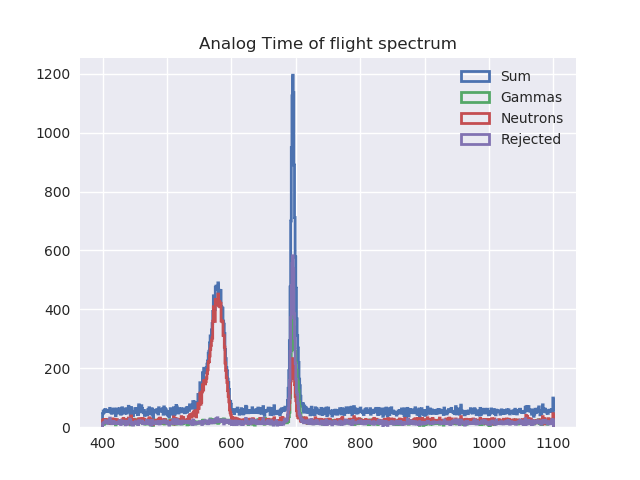
\includegraphics[width=0.8\textwidth]{AnalogResults/tof_psd.pdf}
        \caption[Pulse shape vs. Ttime-of-flight for the analog setup.]{Pulse shape vs. Ttime-of-flight for the analog setup. The dashed white line indicates the PSD cut. Note the logarithmic z-axis.}
    \label{fig:tof_ps_a} 
\end{figure}







\newpage
\section{Digital setup}
\subsection{Neutron Tagging}
Fig.~\ref{fig:tof_d} shows the ToF spectrum acquired by the digital setup. No additional thresholds or normalizations are applied. Gamma-ray and neutron peaks are indicated with arrows. Random coincidences form a flat background. The width of the gamma-flash is again due to the intrinsic time resolution of the detectors. A secondary effect may be the digitization of the pulse. Limited resolution and sampling rate might cause the CFD algorithm to trigger slightly too soon or too late. 

\begin{figure}[ht]
    \centering
        \includegraphics[width=\textwidth]{DigitalResults/tof.pdf}
        \caption[Time of flight spectrum, digital setup.]{The time of flight spectrum. The x-axis denotes the time of flight from source to NE213 detector. The neutron and gamma peaks have been indicated with arrows. The coincidences highlighted in red have been converted to neutron kinetic energies and are shown in the upper right insert.}
        \label{fig:tof_d} 
\end{figure}

The red-shaded flight times in the neutron peak have been used to generate the energy spectrum shown in the insert of Fig.~\ref{fig:tof_d}. The same time and energy ranges used for the analog setup have been used here (31$\--$\SI{68}{\ns} and 1.5$\--$\SI{7}{\MeV}, respectively). The spectrum has far more events at lower energies than the corresponding spectrum for the analog setup, see Fig.~\ref{fig:tof_a}. This is because the digital setup had a lower amplitude threshold than the analog setup. Thus, slower neutrons, which produce current pulses of lower amplitude in the detector may be recorded by the digital setup. The energy spectrum looks qualitatively very similar to the superimposed reference spectrum of Scherzinger. The low energy peak is however located at slightly higher energy and it seems that Scherzinger might have a applied an even lower threshold. 

\subsection{Pulse-shape discrimination}
As with the analog setup, \SI{500}{ns} and \SI{60}{ns} LG and SG integration windows were used to perform PSD.  To linearize the bands the parameters $a$ and $b$ from Eq.~\ref{eq:ps} were chosen as $a$=\SI{287}{\mV\ns} and $b$=\SI{120}{\mV\ns}. In the digital setup, these offsets can be interpreted as voltage offsets of the sampling points. The parameter $a$ corresponds to an voltage offset of 4.79 mV during SG integration of each sample point. Likewise b corresponds to a voltage offset of 0.24 mV per sample point.
The resulting PSD spectrum is shown Fig.~\ref{fig:psd_d}. The Compton edges corresponding to \SI{2.23}{\MeV} amd \SI{4.44}{MeV} gamma-rays are indicated with arrows. A large number of low-energy gamma-rays appear at the bottom left hand corner of the plot due to the lower threshold.
A cut at PS=0.222 separates the neutron and gamma-ray bands. Again, the two distributions overlap at lower deposited energies.

\begin{figure}
    \centering
    \begin{subfigure}[ht]{\textwidth}
    	\centering
        \includegraphics[width=\textwidth]{DigitalResults/psd_d.pdf}
        \caption{}
        \label{fig:psd_d}
    \end{subfigure}
	\begin{subfigure}[ht]{\textwidth}
		\centering
        \includegraphics[width=\textwidth]{DigitalResults/CNNpsd.pdf}
        \caption{}
    	\label{fig:cnn_E} 
    \end{subfigure}
        \caption[Digital pulse-shape discrimination as a function of deposited energy.]{Digital pulse-shape discrimination as a function of deposited energy. The dashed white lines indicate PSD cuts. Structures due to the \SI{2.23}{MeV} and \SI{4.44}{MeV} gamma-rays are indicated. Top panel: CC method. Amplitude threshold is indicated with a red line. Bottom panel: CNN method.}
    \label{fig:ccm_cnn}
\end{figure}

%\subsection{Convolutional Neural Network}
The CNN described in Sec.~\ref{sec:cnn} was also applied to the digitized waveforms. The network was trained to assign a value $y$ between 0 (gamma-ray) and 1 (neutron) to each signal. The result is shown in Fig.~\ref{fig:cnn_E} as a function of deposited energy. As for the CC method, the upper distribution corresponds to neutrons and the lower distribution to gamma-rays. The two bands are separated by a PSD cut at 0.5. To highlight that the distributions overlap slightly at lower energies, the z-axis has been strongly suppressed. The network, trained on events from the two ToF peaks, allows for much cleaner separation between particle species, so that the exact location of the PSD cut is much less critical than in either of the CC implementations.

As for the analog setup, a FoM was calculated based on Gaussian fits to the PS distribution, see Fig. \ref{fig:fom_d}. The FoM parameters are summarized in Table \ref{tab:fom_d}. With a FoM of 0.78, the digital implementation of the CC method provides better results than the analog implementation. For information on the energy dependence of the FoM, see Appendix \ref{ch:appA}.

\begin{table}[h]
\center
\begin{tabular}{|l|l|l|l|l|l|}
\hline
FoM  & Cut   & W$_\gamma$ & Center$_\gamma$ & W$_\textrm{n}$ & Center$_\textrm{n}$ \\ \hline
0.78 & 0.222 & 0.07          & 0.160           & 0.11              & 0.300               \\ \hline
\end{tabular}
\caption{Charge comparison FoM parameters for the digital setup.}
\label{tab:fom_d}
\end{table}

\begin{figure}[h!]
	    \centering
    	    \includegraphics[width=0.8\textwidth]{CompareResults/FOM_digital.pdf}
	    \caption[Pulse-shape figure of merit for the digital setup.]{Pulse-shape figure of merit for the digital setup. The inset shows the pulse-shape parameter as a function of energy.}
   	    \label{fig:fom_d} 
\end{figure}

In Fig.~\ref{fig:tof_cc_tof_cnn}, the digital CC and CNN predictions are shown as functions of ToF. Figure~\ref{fig:tof_digi_cc} shows the narrow gamma-ray distribution and the wider neutron distribution as separated by the CC method. 
The neutron and gamma-ray background forms two slightly separated bands. a gamma-ray band near prediction value 0.15 and a neutron band near 0.3. The two distributions overlap somewhat.  
In Fig.~\ref{fig:tof_digi_cnn}, it can be seen that the CNN method provides a much better separation, although gamma-ray and neutron distributions still overlap slightly near prediction value 0.5. The distribution of random coincidences separate into a gamma-ray band near prediction value 0 and a neutron band near 1.


\begin{figure}
    \centering
    \begin{subfigure}[ht]{\textwidth}
    	\centering
        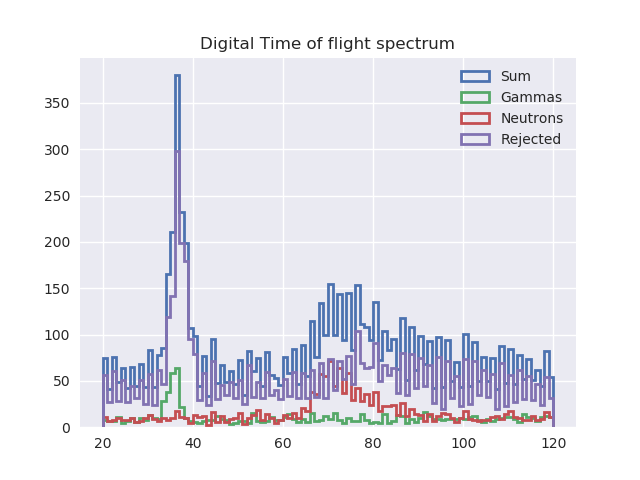
\includegraphics[width=0.8\textwidth]{DigitalResults/tof_psd.pdf}
        \caption{}
        \label{fig:tof_digi_cc}
    \end{subfigure}
	\begin{subfigure}[ht]{\textwidth}
		\centering
        \includegraphics[width=0.8\textwidth]{DigitalResults/CNNtof_psd.pdf}
        \caption{}
        \label{fig:tof_digi_cnn}
    \end{subfigure}
    \caption[Pulse shape vs. time-of-flight for the digital setup.]{Pulse shape vs. Ttime-of-flight for the digital setup. The dashed white line indicates the PSD cut. Note the logarithmic z-axis. Top panel: CC method. Bottom panel: CNN method.}
    \label{fig:tof_cc_tof_cnn}
\end{figure}


\clearpage
\section{Misclassification Rate}\label{sec:comp}


Another way to compare the performance of the PSD methods is by estimating the misclassification. This can be done by evaluating the ToF spectrum in three different regions and comparing the relative number of neutron and gamma-ray labeled events. It is anticipated that the number of gamma-rays identified in a background region containing only random coincidences should be the same as the number of gamma-rays identified in a chosen neighborhood of the neutron time-of-flight peak (after scaling to the widths of the regions). Likewise, the number of neutrons identified at the gamma-flash should correspond to the neutron background expectation. The misclassification of gamma-rays and neutrons, $M_{\gamma}$ and $M_{n}$ respectively can be expressed as

\begin{equation}
	M_\gamma(R_\gamma) = \frac{N_{n}(R_\gamma)-\langle N_n(R_\gamma)\rangle}{N_{\textrm{total}}(R_\gamma)-\langle N_n(R_\gamma)\rangle}
\end{equation}

\begin{equation}
	M_n(R_n) = \frac{N_{\gamma}(R_n)-\langle N_\gamma(R_n)\rangle}{N_{\textrm{total}}(R_n)-\langle N_\gamma(R_n)\rangle},
\end{equation}
where $N_n$ and $N_\gamma$ are the number of neutrons and gamma-rays identified in region $R$ and $N_{\textrm{total}}$ is the sum of $N_n$ and $N_\gamma$. $\langle N_n\rangle$ and $\langle N_\gamma\rangle$ are the expected numbers of neutrons and gamma-rays found by scaling the background rates to the width of $R$.

This definition of misclassification relies on the assumption that the choice of limits for each of the three regions does not seriously impact the results. The neutron peak neighbourhood was set to match the range of neutron energies 1.5-\SI{7}{\MeV} corresponding to $31\--$\SI{68}{ns} and the gamma-flash neighborhood was selected as \SI{5}{\ns} on either side of the gamma-flash center.
It was found that as long as the peaks were contained in the region the misclassifications in percent changed by at most $\pm$0.5\% for the digital setup and at most $\pm$1\% for the analog setup. 


\begin{figure}
    \centering
    \begin{subfigure}[bh]{\textwidth}
   	   	\centering
	    \includegraphics[width=0.85\textwidth]{AnalogResults/ToF_filt.pdf}
    	\caption{PSD cut at PS = 0.259.}
    	\label{fig:ToF_filt_A}
   	\end{subfigure}
    \begin{subfigure}[bh]{\textwidth}
   	    \centering
        \includegraphics[width=0.85\textwidth]{DigitalResults/ToF_filt.pdf}
        \caption{PSD cut at PS=0.222.}
        \label{fig:ToF_filt_D}
    \end{subfigure}
	\begin{subfigure}[bh]{\textwidth}
	    \centering
        \includegraphics[width=0.85\textwidth]{DigitalResults/CNNToF_filt.pdf}
        \caption{PSD cut at prediction = 0.5.}
        \label{fig:ToF_filt_D_CNN}
    \end{subfigure}
	\caption[Filtered time-of-flight spectra for misclassification studies.]{Filtered time-of-flight spectra for misclassification studies.}
    \label{fig:tof_cc_cnn}
\end{figure}

Figure~\ref{fig:tof_cc_cnn} shows the ToF spectrum obtained with the analog setup filtered according to the CC method, as well as the ToF spectrum obtained from the digital setup filtered according to the CC and CNN methods.
For each PSD implementation gamma-ray labeled events are blue, neutron labeled events are red and their intersection purple. 
Ideally, the intersection of the distributions should be flat. However, if there is some systematic misclassification, then the intersection will be above the flat in the ToF spectrum. This may be used to quantify the misclassification of a given PSD implementation.
For the analog setup, a high degree of contamination is evident in the form of the two purple bumps coinciding with the neutron and gamma-ray peaks. This gives an estimated misclassification of 16\% for neutrons and 12\% for gamma-rays. 
The digital setup provides less misclassification with the CC method, at 12\% for neutrons and 3\% for gamma-rays. The much higher misclassification for neutrons implies that the method is biased towards gamma-rays.
The CNN approach reaches the best results with a gamma-ray misclassification of 4\% and a neutron misclassification rate of 5\%.
With a misclassification of nearly the same amount for both neutrons and gamma-rays, the CNN method does not appear to have a strong bias towards either particle species.
The neutron background is found to be nearly the same by the analog and digital CC methods, at 37\% and 38\% respectively. The CNN method finds a significantly higher background of neutron events at 45\%. This together with the high misclassification rates for the CC methods hints at them being biased towards gamma-rays.
The results from all three PSD implementations are summarized in Table \ref{tab:misclas}.

\begin{table}[h]
\center
\begin{tabular}{|l|l|l|l|}
\hline
& \begin{tabular}[c]{@{}l@{}}$\gamma n$-region\\ (\% misclassified)\end{tabular} & \begin{tabular}[c]{@{}l@{}}$\gamma\gamma$-region\\ (\% misclassified)\end{tabular} & \begin{tabular}[c]{@{}l@{}}Background region\\ (\% neutrons)\end{tabular} \\ \hline
\begin{tabular}[c]{@{}l@{}}CC\\ Analog\end{tabular}   & 16                                                                             & 12                                                                                 & 37                                                                        \\ \hline
\begin{tabular}[c]{@{}l@{}}CC\\ Digital\end{tabular}  & 12                                                                             & 3                                                                                  & 38                                                                        \\ \hline
\begin{tabular}[c]{@{}l@{}}CNN\\ Digital\end{tabular} & 5                                                                              & 4                                                                                  & 45                                                                        \\ \hline
\end{tabular}
\caption{Overview of PSD misclasification studies.}
\label{tab:misclas}
\end{table}




\section{Fractional Energy Deposition}

Fig.~\ref{fig:tof_E_d} shows energy deposition in the NE213 detector as a function of ToF, as measured with the digital spectrum. The gamma-flash consisted of gamma-rays that were produced in the de-excitation of $^\mathrm{12}$C (\SI{4.44}{MeV} gamma rays) or in deexcitation of $^\mathrm{234}$U (cascade of low energy gamma rays) as described in the chapter~\ref{ch:1}. Low energy gamma-rays dominate the gamma-flash. This is consistent with the low energy cascade from $\mathrm{234}$U.

\begin{figure}[ht]
    \centering
        \includegraphics{DigitalResults/tof_E.pdf}
        \caption[Time of flight plotted against energy deposition.]{Time of flight plotted against energy deposition.}
    \label{fig:tof_E_d} 
\end{figure}

The neutron distribution shows relationship between ToF and deposited energy. The slowest neutrons have a smaller spread in deposited energy, whereas the faster ones have a much wider spread. This is because the neutron can transfer up to its kinetic energy in a single scattering, as described by Eq.~\ref{eq:scat}. In the NE213 detector the neutron scatters primarily from $^1H$ nuclei. By Eq.~\ref{eq:scat} it is then possible for the neutron to deposit anywhere between 0 and 100\% of its energy, with 0\% implying the neutron missed the nucleus and 100\% implying a head on collision resulting in complete transfer. 
In Fig.~\ref{fig:N_E} this relation is highlighted. 
The central panel shows the deposited energy as a function of neutron kinetic energy. In fact the scintillation light output produced by an NE213 detector is given by Eq.\cite{Scherzinger:2016}, Which approaches a linear shape at as neutron energies rise and the exponential term approaches unity:
\begin{equation}
	\textrm{E}_{deposited} = C\left(  0.83\cdot \textrm{E}_{neutron} - 2.82\cdot\left(  1 - e^{(-0.25\cdot \textrm{E}_{neutron}^{0.93})}  \right)  \right)
	\label{eq:N_E}
\end{equation}
The parameter C depends on the particular detector and can be found through fitting. The red points in Fig \ref{fig:N_E} where found by fitting Gaussians to the deposited energy values of events located in within narrow slices of neutron kinetic energies. Three of the slices along with fits are shown in the top panel. By fitting Eq.~\ref{eq:N_E} to these points The value of $C$ was found to be 0.62. The fact that the fit doesn't match the points so well at lower neutron energies may be due to the amplitude threshold particularly affects the low energy neutrons.

The bottom panel shows the ratio of deposited energy to neutron kinetic energy as a function of neutron kinetic energy. The red points represent the center of Gaussian fitted to the slices. 
%the dotted line at $\sim$1 is the center point of the same type of fit covering all neutron energies. 
The ratio ratio should express the fraction of its kinetic energy that the neutron has transfered. At higher energies it is slightly below 1, suggesting all of the energy is deposited in the detector. At low energies the ratio rises above 1. This unphysical behaviour is likely an effect of the amplitude threshold cutting away neutrons that leave little energy in the detector.

\begin{figure}[ht]
    \centering
        \includegraphics{DigitalResults/N_E.pdf}
        \caption[Neutron kinetic energy and deposited energy.]{Top: Ratio of deposited energy to neutron kinetic energy. Bottom: deposited energy as a function of neutron kinetic energy, along with fits.}
    \label{fig:N_E} 
\end{figure}



\end{document}